\begin{frame}
\frametitle{Learning network protocols despite imperfect assumptions}
\begin{centering}
What are the costs and benefits of designing a new protocol that shares fairly with a legacy sender?
\end{centering}
\end{frame}

\begin{frame}
\frametitle{Imperfect assumptions about the nature of other senders}
\begin{itemize}
\item<1-> \textbf{TCP-Aware} RemyCC: Assumed to run against another \textbf{TCP-Aware} RemyCC half the time, and against TCP NewReno half the time.
\item<2-> \textbf{TCP-Naive} RemyCC: Assumed to run only against another \textbf{TCP-Naive} RemyCC
\end{itemize}
\end{frame}

\begin{frame}
\frametitle{RemyCC competing against itself}
\begin{centering}

\noindent \only<1>{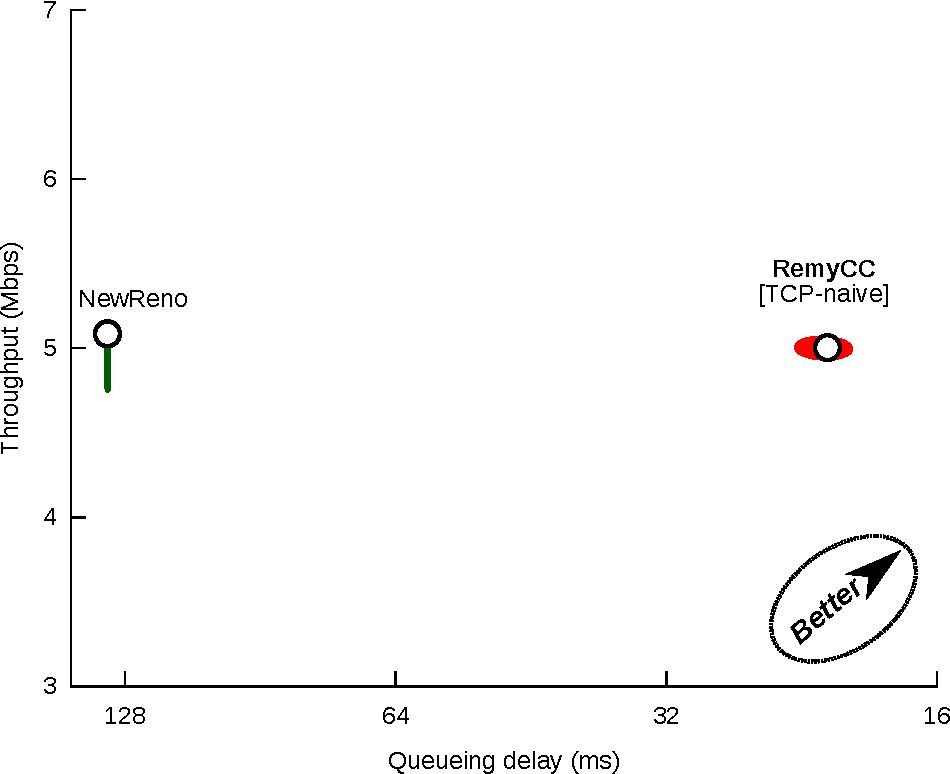
\includegraphics[width=3.3 in]{homo-1.pdf}}\only<2>{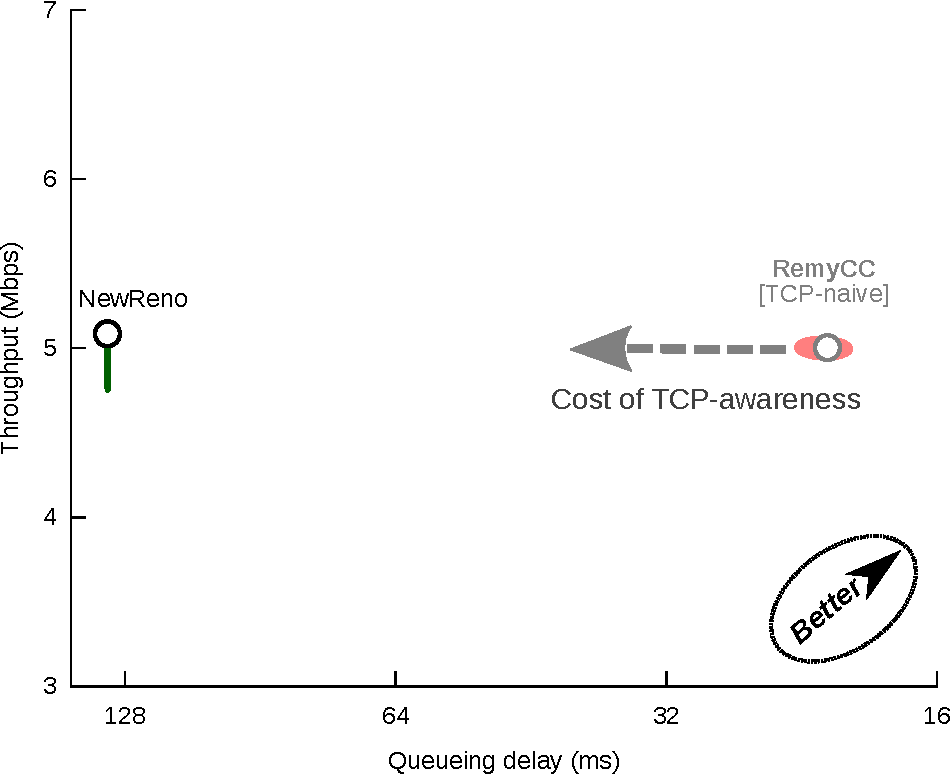
\includegraphics[width=3.3 in]{homo-2.pdf}}\only<3>{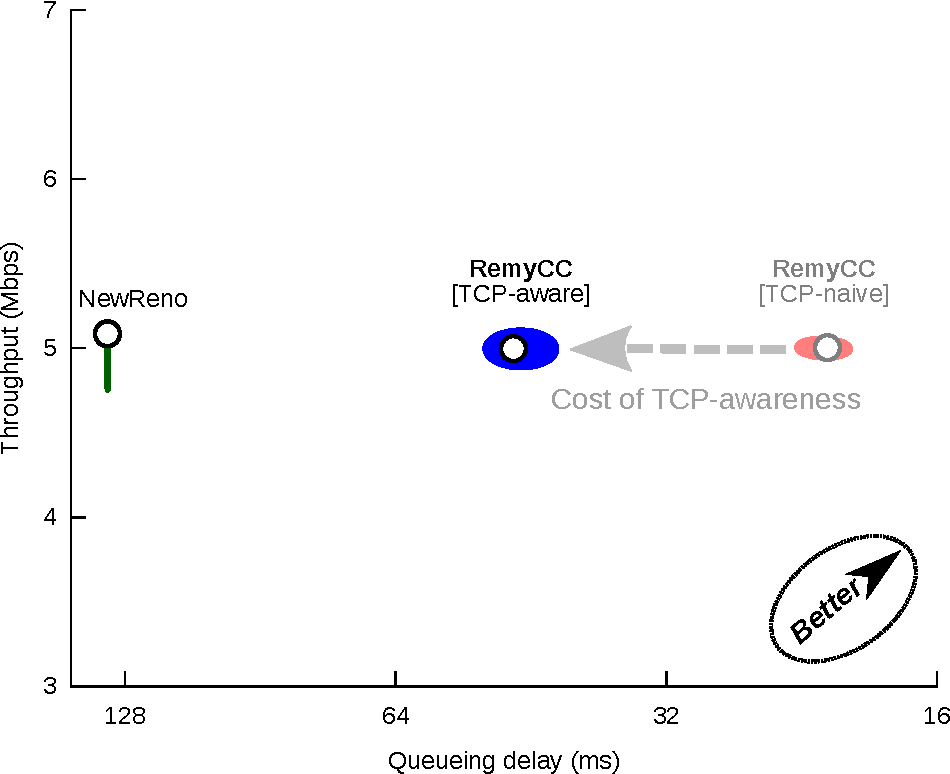
\includegraphics[width=3.3 in]{homo-3.pdf}}

\end{centering}
\end{frame}

\begin{frame}
\frametitle{RemyCC competing against TCP NewReno}
\begin{centering}

\noindent \only<1>{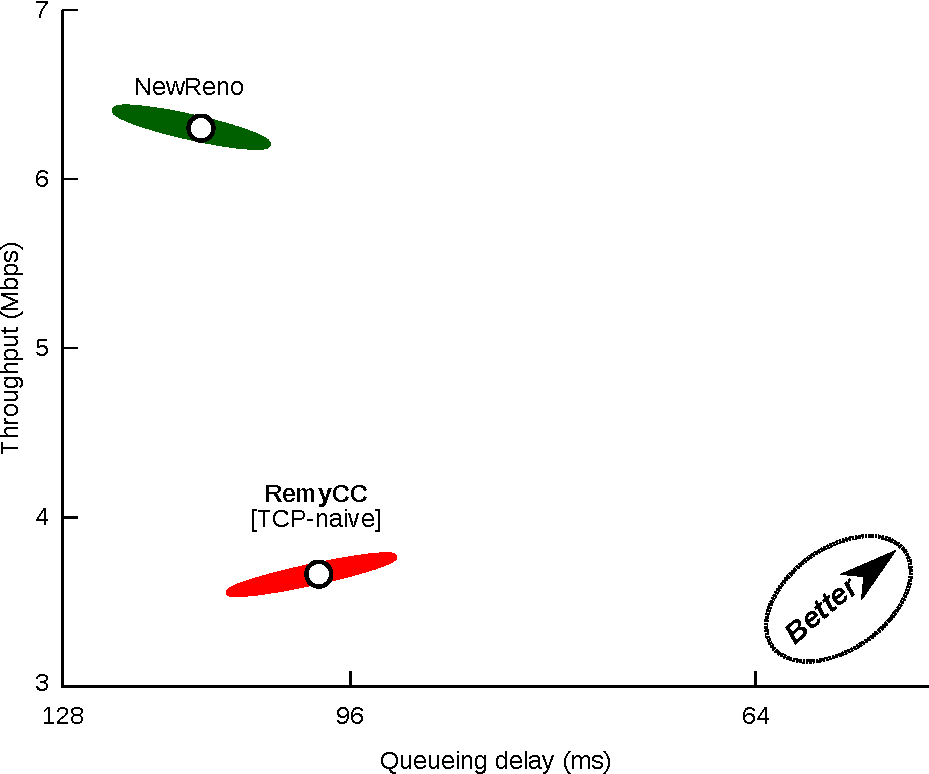
\includegraphics[width=3.3 in]{hetero-1.pdf}}\only<2>{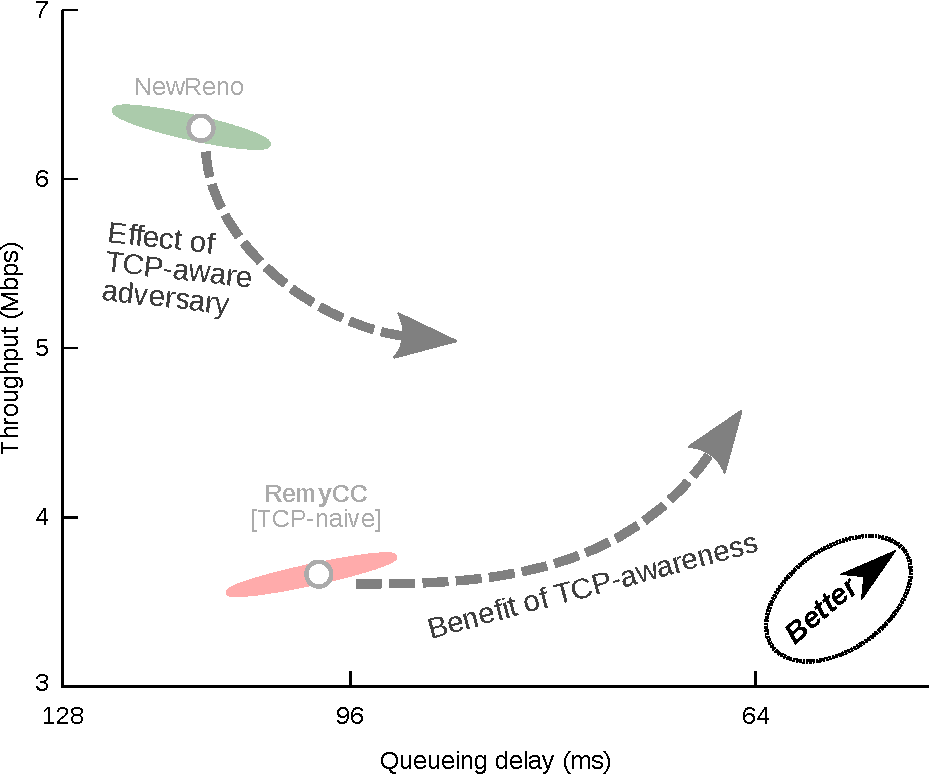
\includegraphics[width=3.3 in]{hetero-2.pdf}}\only<3>{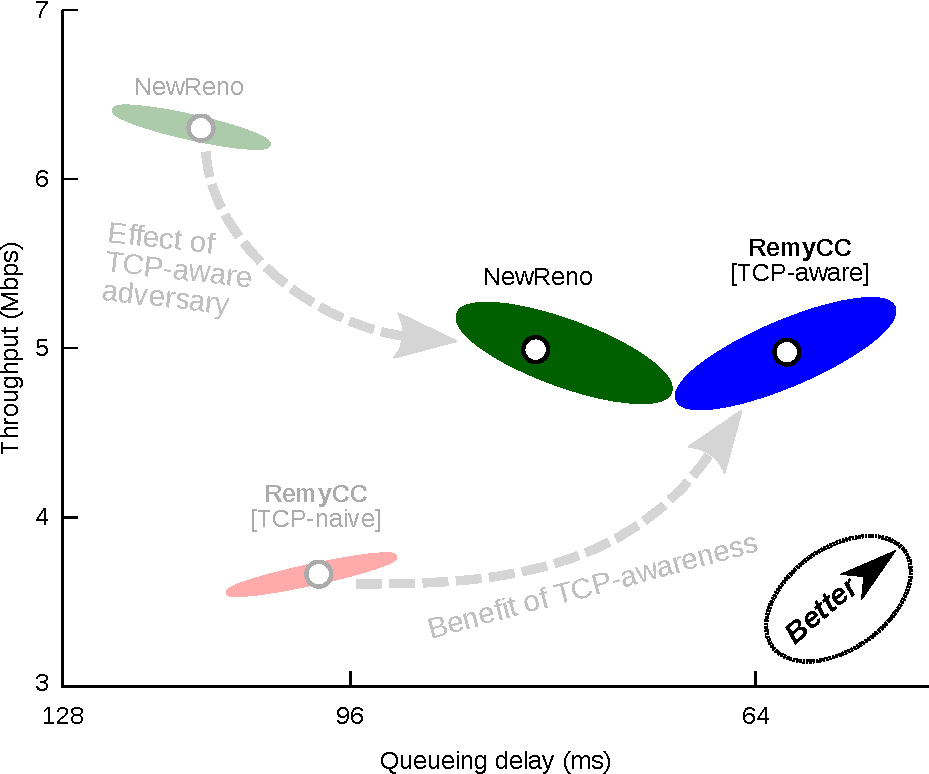
\includegraphics[width=3.3 in]{hetero-3.pdf}}

\only<4>{TCP awareness benefits you when needed, costs if you don't}
\end{centering}
\end{frame}
